\begin{figure}[!htb]
  \begin{center}
    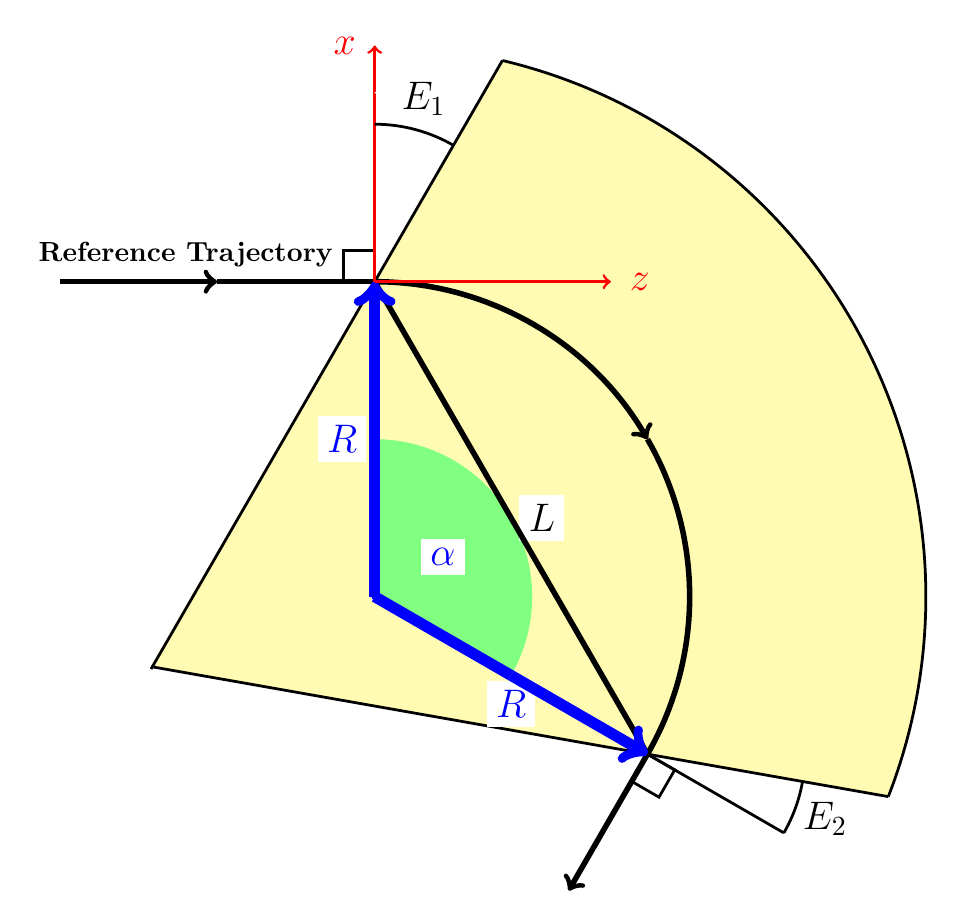
\begin{tikzpicture}[scale=4]
      % Draw magnet shape.
      \filldraw[yellow!30!white] (-0.709667,-1.22216292)
      -- (0.4055127895,0.702368754) arc (76.6015496:-21.2704331:1.75)
      -- (-0.709667,-1.22216292);

      \draw[line width=1pt, rotate around={-30:(0.0,0.0)}] (0,-1.42) -- (0,0.811025579);
      \draw[line width=1pt] (0.40551279,0.70236875) arc (76.6015496:-21.2704331:1.75);
      \draw[line width=1pt] (1.6307875,-1.6348482) -- (-0.709667,-1.22216292);

      % Now draw squares indicating 90 degree angles to bend radius at entrance and exit.
      \draw[line width=1pt] (0.0,0.0) rectangle (-0.1,0.1);
      \draw[line width=1pt,xshift=0.8660254cm,yshift=-1.5cm,rotate around={60:(0.0,0.0)}]
      (-0.1,-0.1) rectangle (0.0,0.0);

      % Draw reference particle path.
      \draw[white] (-1.1,0.0) -- (-0.6,0.0)
      node[above=2pt] {\textbf{\color{black}Reference Trajectory}};
      \draw[arrows=->,line width=2pt] (-1.0,0.0) -- (-0.5,0.0);
      \draw[line width=2pt] (-0.5,0.0) -- (0.0,0.0);
      \draw[arrows=->,line width=2pt] (0.0,0.0) arc (90:30:1.0);
      \draw[line width=2pt] (0.8660254,-0.5) arc (30:-30:1.0);
      \draw[arrows=->,line width=2pt] (0.8660254,-1.5) -- (0.6160254,-1.9330127);

      % Draw bend angle.
      \fill[green!50!white] (0.0,-1.0) -- (0.0,-0.5) arc (90:-30:0.5) -- (0.0,-1.0);
      \draw[green!50!white] (0.0,-0.75) arc (90:30:0.25)
      node[fill=white] {\Large{\textbf{\color{blue}$\alpha$}}};

      % Label chord length.
      \draw[line width=2pt] (0.0,0.0) -- (0.4330127,-0.75)
      node[fill=white,right=2pt] {\Large{\textbf{\color{black}$L$}}};
      \draw[line width=2pt] (0.4330127,-0.75) -- (0.8660254,-1.5);

      % Draw bend radii at entrance and exit.
      \draw[blue,line width=4pt] (0.0,-1.0) -- (0.0,-0.5)
      node[blue,left=1pt,fill=white] {\Large{\textbf{$R$}}};
      \draw[arrows=->,blue,line width=4pt] (0.0,-0.5) -- (0.0,0.0);

      \draw[blue,line width=4pt] (0.0,-1.0) -- (0.4330127,-1.25)
      node[below=0pt,fill=white] {\Large{\textbf{$R$}}};
      \draw[arrows=->,blue,line width=4pt] (0.4330127,-1.25) -- (0.8660254,-1.5);
      \filldraw[blue] (0.0,-1.0) circle (0.25pt);

     % Draw reference axes.
      \draw[red,arrows=->,line width=1pt] (0.0,0.0) -- (0.0,0.75) node[left=3pt] {\Large{\textbf{$x$}}};
      \draw[red,arrows=->,line width=1pt] (0.0,0.0) -- (0.75,0.0) node[right=3pt] {\Large{\textbf{$z$}}};

      % Label entrance angle.
      \draw[line width=1pt] (0.0,0.5) arc (90:60:0.5);
      \draw[white] (0.0,0.6) arc (90:75:0.6) node[] {\Large{\textbf{\color{black}$E_{1}$}}};

      % Label exit angle.
      \draw[line width=1pt,xshift=0.8660254cm,yshift=-1.5cm,rotate around={-120:(0.0,0.0)}] (0.0,0.0) -- (0.0,0.5);
      \draw[line width=1pt,xshift=0.8660254cm,yshift=-1.5cm,rotate around={-120:(0.0,0.0)}] (0.0,0.5) arc(90:110:0.5);
      \draw[white,xshift=0.8660254cm,yshift=-1.5cm,rotate around={-120:(0.0,0.0)}] (0.0, 0.6) arc (90:100:0.6)
      node[] {\Large{\textbf{\color{black}$E_{2}$}}};

    \end{tikzpicture}
  \end{center}
  \caption{Illustration of a general sector bend (\keyword{SBEND}) with a positive bend angle $\alpha$. In this example
    the entrance and exit edge angles $E_{1}$ and $E_{2}$ have positive values. For a positively charge particle,
    the magnetic field is directed out of the page.}
  \label{fig:sbend}
\end{figure}